%===============================================================================
% LaTeX sjabloon voor de bachelorproef toegepaste informatica aan HOGENT
% Meer info op https://github.com/HoGentTIN/latex-hogent-report
%===============================================================================

\documentclass[dutch,dit,thesis]{hogentreport}

% TODO:
% - If necessary, replace the option `dit`' with your own department!
%   Valid entries are dbo, dbt, dgz, dit, dlo, dog, dsa, soa
% - If you write your thesis in English (remark: only possible after getting
%   explicit approval!), remove the option "dutch," or replace with "english".

\usepackage{lipsum} % For blind text, can be removed after adding actual content

%% Pictures to include in the text can be put in the graphics/ folder
\graphicspath{{graphics/}}

%% For source code highlighting, requires pygments to be installed
%% Compile with the -shell-escape flag!
\usepackage[section]{minted}
%% If you compile with the make_thesis.{bat,sh} script, use the following
%% import instead:
%% \usepackage[section,outputdir=../output]{minted}
\usemintedstyle{solarized-light}
\definecolor{bg}{RGB}{253,246,227} %% Set the background color of the codeframe

%% Change this line to edit the line numbering style:
\renewcommand{\theFancyVerbLine}{\ttfamily\scriptsize\arabic{FancyVerbLine}}

%% Macro definition to load external java source files with \javacode{filename}:
\newmintedfile[javacode]{java}{
    bgcolor=bg,
    fontfamily=tt,
    linenos=true,
    numberblanklines=true,
    numbersep=5pt,
    gobble=0,
    framesep=2mm,
    funcnamehighlighting=true,
    tabsize=4,
    obeytabs=false,
    breaklines=true,
    mathescape=false
    samepage=false,
    showspaces=false,
    showtabs =false,
    texcl=false,
}

% Other packages not already included can be imported here

%%---------- Document metadata -------------------------------------------------
% TODO: Replace this with your own information
\author{Ernst Aarden}
\supervisor{Dhr. F. Van Houte}
\cosupervisor{Mevr. S. Beeckman}
\title[Optionele ondertitel]%
    {Titel van de bachelorproef}
\academicyear{\advance\year by -1 \the\year--\advance\year by 1 \the\year}
\examperiod{1}
\degreesought{\IfLanguageName{dutch}{Professionele bachelor in de toegepaste informatica}{Bachelor of applied computer science}}
\partialthesis{false} %% To display 'in partial fulfilment'
%\institution{Internshipcompany BVBA.}

%% Add global exceptions to the hyphenation here
\hyphenation{back-slash}

%% The bibliography (style and settings are  found in hogentthesis.cls)
\addbibresource{bachproef.bib}            %% Bibliography file
\addbibresource{../voorstel/voorstel.bib} %% Bibliography research proposal
\defbibheading{bibempty}{}

%% Prevent empty pages for right-handed chapter starts in twoside mode
\renewcommand{\cleardoublepage}{\clearpage}

\renewcommand{\arraystretch}{1.2}

%% Content starts here.
\begin{document}

%---------- Front matter -------------------------------------------------------

\frontmatter

\hypersetup{pageanchor=false} %% Disable page numbering references
%% Render a Dutch outer title page if the main language is English
\IfLanguageName{english}{%
    %% If necessary, information can be changed here
    \degreesought{Professionele Bachelor toegepaste informatica}%
    \begin{otherlanguage}{dutch}%
       \maketitle%
    \end{otherlanguage}%
}{}

%% Generates title page content
\maketitle
\hypersetup{pageanchor=true}

%%=============================================================================
%% Voorwoord
%%=============================================================================

\chapter*{\IfLanguageName{dutch}{Woord vooraf}{Preface}}%
\label{ch:voorwoord}

%% TODO:
%% Het voorwoord is het enige deel van de bachelorproef waar je vanuit je
%% eigen standpunt (``ik-vorm'') mag schrijven. Je kan hier bv. motiveren
%% waarom jij het onderwerp wil bespreken.
%% Vergeet ook niet te bedanken wie je geholpen/gesteund/... heeft

\lipsum[1-2]
%%=============================================================================
%% Samenvatting
%%=============================================================================

% TODO: De "abstract" of samenvatting is een kernachtige (~ 1 blz. voor een
% thesis) synthese van het document.
%
% Een goede abstract biedt een kernachtig antwoord op volgende vragen:
%
% 1. Waarover gaat de bachelorproef?
% 2. Waarom heb je er over geschreven?
% 3. Hoe heb je het onderzoek uitgevoerd?
% 4. Wat waren de resultaten? Wat blijkt uit je onderzoek?
% 5. Wat betekenen je resultaten? Wat is de relevantie voor het werkveld?
%
% Daarom bestaat een abstract uit volgende componenten:
%
% - inleiding + kaderen thema
% - probleemstelling
% - (centrale) onderzoeksvraag
% - onderzoeksdoelstelling
% - methodologie
% - resultaten (beperk tot de belangrijkste, relevant voor de onderzoeksvraag)
% - conclusies, aanbevelingen, beperkingen
%
% LET OP! Een samenvatting is GEEN voorwoord!

%%---------- Nederlandse samenvatting -----------------------------------------
%
% TODO: Als je je bachelorproef in het Engels schrijft, moet je eerst een
% Nederlandse samenvatting invoegen. Haal daarvoor onderstaande code uit
% commentaar.
% Wie zijn bachelorproef in het Nederlands schrijft, kan dit negeren, de inhoud
% wordt niet in het document ingevoegd.

\IfLanguageName{english}{%
\selectlanguage{dutch}
\chapter*{Samenvatting}

\selectlanguage{english}
}{}

%%---------- Samenvatting -----------------------------------------------------
% De samenvatting in de hoofdtaal van het document

\chapter*{\IfLanguageName{dutch}{Samenvatting}{Abstract}}

Tegenwoordig is er een exponentiële groei in het gebruik van e-commerce webshops. De onderliggende database speelt hierbij een belangrijke rol. Om developers binnen bedrijven in de toekomst te kunnen ondersteunen bij hun keuze voor een databaseoplossing, zal er een onderzoek gevoerd worden naar de meest geschikte database oplossing voor een e-commerce webshop in de mode-industrie. Het onderzoek richt zich op het evalueren van vijf verschillende database oplossingen. De focus zal hierbij gelegd worden op de prestaties en kosten van de desbetreffende databases. Het onderzoek zelf zal onderverdeeld worden in zes verschillende fases. In eerste instantie zal er een literatuurstudie worden gevoerd. In de stand van zaken zal informatie worden gegeven over de verschillende soorten databases die er bestaan en zal nagegaan worden welke databases momenteel gebruikt worden door het bedrijf Aware. Na de literatuurstudie volgt een requirements analyse waarin de functionele- en niet-functionele requirements voor dergelijk databasesysteem besproken worden. In een volgende stap wordt een short list van vijf verschillende databases opgesteld. Vervolgens wordt een vergelijkende studie van deze vijf databases uitgevoerd. Deze studie bestaat enkel uit gevonden literatuur en technische gegevens van deze databases. Nadien volgt een Proof of Concept (PoC) waarin elk van deze databases uitgetest wordt. In laatste instantie wordt op basis van de vergelijkende studie en de resultaten van de PoC een besluit getrokken die weergegeven wordt in de conclusie.

\vspace{5mm}

Op basis van dit onderzoek kunnen we besluiten dat de keuze van de database deels afhankelijk is van de voorkeuren van de developer. Indien geopteerd wordt voor een SQL databasesysteem wordt ClickHouse aangeraden. Indien de developer een voorkeur heeft voor een NoSQL database wordt vooral MongoDB aangeraden.

%---------- Inhoud, lijst figuren, ... -----------------------------------------

\tableofcontents

% In a list of figures, the complete caption will be included. To prevent this,
% ALWAYS add a short description in the caption!
%
%  \caption[short description]{elaborate description}
%
% If you do, only the short description will be used in the list of figures

\listoffigures

% If you included tables and/or source code listings, uncomment the appropriate
% lines.
%\listoftables
%\listoflistings

% Als je een lijst van afkortingen of termen wil toevoegen, dan hoort die
% hier thuis. Gebruik bijvoorbeeld de ``glossaries'' package.
% https://www.overleaf.com/learn/latex/Glossaries

%---------- Kern ---------------------------------------------------------------

\mainmatter{}

% De eerste hoofdstukken van een bachelorproef zijn meestal een inleiding op
% het onderwerp, literatuurstudie en verantwoording methodologie.
% Aarzel niet om een meer beschrijvende titel aan deze hoofdstukken te geven of
% om bijvoorbeeld de inleiding en/of stand van zaken over meerdere hoofdstukken
% te verspreiden!

%%=============================================================================
%% Inleiding
%%=============================================================================

\chapter{\IfLanguageName{dutch}{Inleiding}{Introduction}}%
\label{ch:inleiding}

De inleiding moet de lezer net genoeg informatie verschaffen om het onderwerp te begrijpen en in te zien waarom de onderzoeksvraag de moeite waard is om te onderzoeken. In de inleiding ga je literatuurverwijzingen beperken, zodat de tekst vlot leesbaar blijft. Je kan de inleiding verder onderverdelen in secties als dit de tekst verduidelijkt. Zaken die aan bod kunnen komen in de inleiding~\autocite{Pollefliet2011}:

\begin{itemize}
  \item context, achtergrond
  \item afbakenen van het onderwerp
  \item verantwoording van het onderwerp, methodologie
  \item probleemstelling
  \item onderzoeksdoelstelling
  \item onderzoeksvraag
  \item \ldots
\end{itemize}

\section{\IfLanguageName{dutch}{Probleemstelling}{Problem Statement}}%
\label{sec:probleemstelling}

Uit je probleemstelling moet duidelijk zijn dat je onderzoek een meerwaarde heeft voor een concrete doelgroep. De doelgroep moet goed gedefinieerd en afgelijnd zijn. Doelgroepen als ``bedrijven,'' ``KMO's'', systeembeheerders, enz.~zijn nog te vaag. Als je een lijstje kan maken van de personen/organisaties die een meerwaarde zullen vinden in deze bachelorproef (dit is eigenlijk je steekproefkader), dan is dat een indicatie dat de doelgroep goed gedefinieerd is. Dit kan een enkel bedrijf zijn of zelfs één persoon (je co-promotor/opdrachtgever).

\section{\IfLanguageName{dutch}{Onderzoeksvraag}{Research question}}%
\label{sec:onderzoeksvraag}

Wees zo concreet mogelijk bij het formuleren van je onderzoeksvraag. Een onderzoeksvraag is trouwens iets waar nog niemand op dit moment een antwoord heeft (voor zover je kan nagaan). Het opzoeken van bestaande informatie (bv. ``welke tools bestaan er voor deze toepassing?'') is dus geen onderzoeksvraag. Je kan de onderzoeksvraag verder specifiëren in deelvragen. Bv.~als je onderzoek gaat over performantiemetingen, dan 

\section{\IfLanguageName{dutch}{Onderzoeksdoelstelling}{Research objective}}%
\label{sec:onderzoeksdoelstelling}

Wat is het beoogde resultaat van je bachelorproef? Wat zijn de criteria voor succes? Beschrijf die zo concreet mogelijk. Gaat het bv.\ om een proof-of-concept, een prototype, een verslag met aanbevelingen, een vergelijkende studie, enz.

\section{\IfLanguageName{dutch}{Opzet van deze bachelorproef}{Structure of this bachelor thesis}}%
\label{sec:opzet-bachelorproef}

% Het is gebruikelijk aan het einde van de inleiding een overzicht te
% geven van de opbouw van de rest van de tekst. Deze sectie bevat al een aanzet
% die je kan aanvullen/aanpassen in functie van je eigen tekst.

De rest van deze bachelorproef is als volgt opgebouwd:

In Hoofdstuk~\ref{ch:stand-van-zaken} wordt een overzicht gegeven van de stand van zaken binnen het onderzoeksdomein, op basis van een literatuurstudie.

In Hoofdstuk~\ref{ch:methodologie} wordt de methodologie toegelicht en worden de gebruikte onderzoekstechnieken besproken om een antwoord te kunnen formuleren op de onderzoeksvragen.

% TODO: Vul hier aan voor je eigen hoofstukken, één of twee zinnen per hoofdstuk

In Hoofdstuk~\ref{ch:conclusie}, tenslotte, wordt de conclusie gegeven en een antwoord geformuleerd op de onderzoeksvragen. Daarbij wordt ook een aanzet gegeven voor toekomstig onderzoek binnen dit domein.
\chapter{\IfLanguageName{dutch}{Stand van zaken}{State of the art}}%
\label{ch:stand-van-zaken}

% Tip: Begin elk hoofdstuk met een paragraaf inleiding die beschrijft hoe
% dit hoofdstuk past binnen het geheel van de bachelorproef. Geef in het
% bijzonder aan wat de link is met het vorige en volgende hoofdstuk.

% Pas na deze inleidende paragraaf komt de eerste sectiehoofding.

Dit hoofdstuk bevat je literatuurstudie. De inhoud gaat verder op de inleiding, maar zal het onderwerp van de bachelorproef *diepgaand* uitspitten. De bedoeling is dat de lezer na lezing van dit hoofdstuk helemaal op de hoogte is van de huidige stand van zaken (state-of-the-art) in het onderzoeksdomein. Iemand die niet vertrouwd is met het onderwerp, weet nu voldoende om de rest van het verhaal te kunnen volgen, zonder dat die er nog andere informatie moet over opzoeken \autocite{Pollefliet2011}.

Je verwijst bij elke bewering die je doet, vakterm die je introduceert, enz.\ naar je bronnen. In \LaTeX{} kan dat met het commando \texttt{$\backslash${textcite\{\}}} of \texttt{$\backslash${autocite\{\}}}. Als argument van het commando geef je de ``sleutel'' van een ``record'' in een bibliografische databank in het Bib\LaTeX{}-formaat (een tekstbestand). Als je expliciet naar de auteur verwijst in de zin (narratieve referentie), gebruik je \texttt{$\backslash${}textcite\{\}}. Soms is de auteursnaam niet expliciet een onderdeel van de zin, dan gebruik je \texttt{$\backslash${}autocite\{\}} (referentie tussen haakjes). Dit gebruik je bv.~bij een citaat, of om in het bijschrift van een overgenomen afbeelding, broncode, tabel, enz. te verwijzen naar de bron. In de volgende paragraaf een voorbeeld van elk.

\textcite{Knuth1998} schreef een van de standaardwerken over sorteer- en zoekalgoritmen. Experten zijn het erover eens dat cloud computing een interessante opportuniteit vormen, zowel voor gebruikers als voor dienstverleners op vlak van informatietechnologie~\autocite{Creeger2009}.

Let er ook op: het \texttt{cite}-commando voor de punt, dus binnen de zin. Je verwijst meteen naar een bron in de eerste zin die erop gebaseerd is, dus niet pas op het einde van een paragraaf.

\lipsum[7-20]

%%=============================================================================
%% Methodologie
%%=============================================================================

\chapter{\IfLanguageName{dutch}{Methodologie}{Methodology}}%
\label{ch:methodologie}

%% TODO: In dit hoofstuk geef je een korte toelichting over hoe je te werk bent
%% gegaan. Verdeel je onderzoek in grote fasen, en licht in elke fase toe wat
%% de doelstelling was, welke deliverables daar uit gekomen zijn, en welke
%% onderzoeksmethoden je daarbij toegepast hebt. Verantwoord waarom je
%% op deze manier te werk gegaan bent.
%% 
%% Voorbeelden van zulke fasen zijn: literatuurstudie, opstellen van een
%% requirements-analyse, opstellen long-list (bij vergelijkende studie),
%% selectie van geschikte tools (bij vergelijkende studie, "short-list"),
%% opzetten testopstelling/PoC, uitvoeren testen en verzamelen
%% van resultaten, analyse van resultaten, ...
%%
%% !!!!! LET OP !!!!!
%%
%% Het is uitdrukkelijk NIET de bedoeling dat je het grootste deel van de corpus
%% van je bachelorproef in dit hoofstuk verwerkt! Dit hoofdstuk is eerder een
%% kort overzicht van je plan van aanpak.
%%
%% Maak voor elke fase (behalve het literatuuronderzoek) een NIEUW HOOFDSTUK aan
%% en geef het een gepaste titel.

\lipsum[21-25]



% Voeg hier je eigen hoofdstukken toe die de ``corpus'' van je bachelorproef
% vormen. De structuur en titels hangen af van je eigen onderzoek. Je kan bv.
% elke fase in je onderzoek in een apart hoofdstuk bespreken.

%\input{...}
%\input{...}
%...

%%=============================================================================
%% Conclusie
%%=============================================================================

\chapter{Conclusie}%
\label{ch:conclusie}

% TODO: Trek een duidelijke conclusie, in de vorm van een antwoord op de
% onderzoeksvra(a)g(en). Wat was jouw bijdrage aan het onderzoeksdomein en
% hoe biedt dit meerwaarde aan het vakgebied/doelgroep? 
% Reflecteer kritisch over het resultaat. In Engelse teksten wordt deze sectie
% ``Discussion'' genoemd. Had je deze uitkomst verwacht? Zijn er zaken die nog
% niet duidelijk zijn?
% Heeft het onderzoek geleid tot nieuwe vragen die uitnodigen tot verder 
%onderzoek?

\lipsum[76-80]



%---------- Bijlagen -----------------------------------------------------------

\appendix

\chapter{Onderzoeksvoorstel}

Het onderwerp van deze bachelorproef is gebaseerd op een onderzoeksvoorstel dat vooraf werd beoordeeld door de promotor. Dat voorstel is opgenomen in deze bijlage.

%% TODO: 
%\section*{Samenvatting}

% Kopieer en plak hier de samenvatting (abstract) van je onderzoeksvoorstel.

% Verwijzing naar het bestand met de inhoud van het onderzoeksvoorstel
%---------- Inleiding ---------------------------------------------------------

\section{Introductie}%
\label{sec:introductie}

De keuze van de juiste databaseoplossing is van belang voor het succes van online mode-e-commerce platformen. Dit onderzoek is gericht op het identificeren van een databasearchitectuur die een balans biedt tussen prestaties en kostenbeheersing voor kleine tot middelgrote mode-e-commerce platformen. Gedurende een periode van vier maanden zullen verschillende databasebeheersystemen geëvalueerd worden op basis van de reactietijd, doorvoersnelheid en operationele kosten. Het einddoel van dit onderzoek is om een gestructureerde benadering te realiseren die mode-ondernemers kan helpen bij het maken van beslissingen op basis van data voor hun e-commerce systemen. De resultaten zullen een duidelijker beeld geven over hoe kleinere e-commerce ondernemingen zich kunnen schalen en klanttevredenheid kunnen verbeteren door de selectie van de gepaste technologieën. Hiermee wordt ook meteen volgende onderzoeksvraag opgelost: ``Hoe evalueren verschillende databaseoplossingen op het gebied van prestaties en kosten voor het ondersteunen van een kleine e-commerce website in de mode-industrie, binnen een onderzoeksperiode van vier maanden?''.

%---------- Stand van zaken ---------------------------------------------------

\section{Literatuurstudie}%
\label{sec:literatuurstudie}
In deze studie wordt, binnen een onderzoeksperiode van vier maanden, nagegaan welke
verschillende databaseoplossingen het meest geschikt zijn op gebied van prestaties en kosten voor
het ondersteunen van kleine e-commerce websites in de mode-industrie. Het onderzoek richt zich op
het identificeren van de meest geschikte databasesystemen die zowel efficiënt als kosteneffectief
zijn voor kleinere ondernemingen in de snel veranderende modebranche.

Voor het opbouwen van een succesvol e-commerce platform in de modebranche is het kiezen van
een concrete databaseoplossing van cruciaal belang. Tegenwoordig is het maken van die keuze
echter niet meer vanzelfsprekend. Bij het maken van een keuze moet er rekening gehouden worden
met verschillende belangrijke factoren, zoals bijvoorbeeld de kosten die deze oplossing met zich
meebrengt, de betrouwbaarheid van de database, de schaalbaarheid en de prestaties. Voor het
bouwen van een moderne e-commerce website, en meer specifiek één in de mode-industrie is er
vooral nood aan een databaseoplossing waarbij er snel en efficiënt omgegaan kan worden met grote
hoeveelheden aan ongestructureerde data en dit terwijl er een optimale gebruikerservaring
behouden wordt. Hiernaast is het ook belangrijk dat deze oplossing kosteneffectief is zodat kleine
bedrijven geen last ondervinden van te hoge operationele kosten.

De populaire NoSQL-database, MongoDB, die bekend staat voor zijn vermogen om flexibel om te
gaan met ongestructureerde data is daarom mogelijks een interessante keuze voor dynamische en
data-intensieve e-commerce platforms~\autocite{Inetum2022}. MongoDB's document-
georiënteerde benadering maakt het geschikt voor toepassingen die snelle ontwikkeling vereisen en
daarbovenop levert het goede resultaten in het omgaan met grote volumes aan diverse data. Echter,
kunnen de kosten voor het gebruik van MongoDB variëren, afhankelijk van de schaal en de vereiste
functionaliteiten, wat een aandachtspunt is voor kostengevoelige projecten.

Anderzijds is er ook de mogelijkheid om gebruik te maken van een traditionele SQL-database, zoals
MySQL of PostgreSQL. Deze databases staan bekend om hun robuustheid bij het verwerken van
gestructureerde gegevens en hun complexe zoekopdrachten. Volgens \textcite{Solarwinds} zijn traditionele databases met name geschikt voor het uitvoeren van transactie-intensieve applicaties,
zoals die vaak voorkomen in e-commerceomgevingen. Ze bieden een hoge betrouwbaarheid en sterke consistentie, maar zijn mogelijk minder flexibel in termen van schemawijzigingen. Ze kunnen ook uitdagingen opleveren bij het opschalen naar grote hoeveelheden ongestructureerde gegevens.

Naast traditionele SQL- of NoSQL-databases kan ook gebruik worden gemaakt van een Graph-database. Zowel ~\textcite{AWS} als ~\textcite{Foote2023} benadrukken dat Graph-databases een flexibeler platform bieden voor het detecteren en tot stand brengen van verbindingen en relaties. Door hun ontwerp zijn grafische databases vaak ook sneller in het presenteren van relaties dan relationele databases. Volgens ~\textcite{AWS} biedt een grafische database echter alleen meerwaarde voor datasets met sterke onderlinge verbindingen en de daarbij behorende analyses, waarbij verborgen en schijnbare relaties moeten worden onthuld.

Een mogelijke oplossing om zowel flexibel om te kunnen gaan met ongestructureerde data als
gestructureerde transactiedata is door gebruik te maken van een hybride benadering ~\autocite{DevX2023}. Dit laat toe om
gebruik te maken van een NoSQL database voor het beheer van dynamische, ongestructureerde
data, zoals MongoDB, en het gebruik van een SQL-database voor de gestructureerde transactiedata
zoals MySQL of PostgreSQL. Hierdoor zouden niet alleen de prestaties worden geoptimaliseerd maar
zouden ook de kosten beheerst kunnen worden. Dit is essentieel voor kleine bedrijven in een
competitieve markt.

Het uiteindelijke doel bestaat erin om een databaseoplossing te vinden die een optimale balans biedt
tussen de kosten en prestaties enerzijds en de flexibiliteit waarmee ingespeeld kan worden op de
veranderende behoeften van de mode-industrie anderzijds.

% Voor literatuurverwijzingen zijn er twee belangrijke commando's:
% \autocite{KEY} => (Auteur, jaartal) Gebruik dit als de naam van de auteur
%   geen onderdeel is van de zin.
% \textcite{KEY} => Auteur (jaartal)  Gebruik dit als de auteursnaam wel een
%   functie heeft in de zin (bv. ``Uit onderzoek door Doll & Hill (1954) bleek
%   ...'')



%---------- Methodologie ------------------------------------------------------
\section{Methodologie}
\label{sec:methodologie}

\subsection{Fase 1: Literatuurstudie}
\label{subsec:literatuurstudie}
In de eerste fase zal er een uitgebreide literatuurstudie uitgevoerd worden om de huidige stand van zaken in database technologieën voor e-commerce platformen in kaart te brengen. Er zullen relevante academische papers, technische documentatie, en marktanalyses bestudeerd worden. Deze fase zal tussen de drie en vier weken duren.
\textbf{Deliverables:} Een overzicht van bestaande databaseoplossingen en een samenvatting van relevante onderzoeksartikelen.

\subsection{Fase 2: Requirements-analyse}
\label{subsec:requirementsanalyse}
In de tweede fase zal er onderzocht worden wat de functionele en niet-functionele eisen zijn voor kleine tot middelgrote mode-e-commerce platformen. Dit zal gedaan worden door in gesprek te gaan of het sturen van mails met stakeholders in kleine tot middelgrote mode-e-commerce platformen. Deze fase zal ongeveer één à twee weken duren.

\textbf{Deliverables:} Een lijst van requirements voor de databasearchitectuur.

\subsection{Fase 3: Experimenteel Ontwerp}
\label{subsec:experimenteelontwerp}
In deze fase zal een reeks experimenten opgezet worden om verschillende databasebeheersystemen te evalueren. Deze experimenten zullen zich richten op prestatie-indicatoren zoals reactietijd en doorvoersnelheid. Deze fase zal ongeveer één à twee weken duren.

\textbf{Deliverables:} Een experimenteel plan en testprotocollen.

\subsection{Fase 4: Data-analyse}
\label{subsec:dataanalyse}
In fase vier zal de verzamelde data uit de experimenten geanalyseerd worden met statistische software om significante patronen en verschillen te identificeren. Deze fase zal ongeveer één à twee weken duren.

\textbf{Deliverables:} Een statistisch onderbouwd rapport met de bevindingen uit de experimenten.

\subsection{Fase 5: Vergelijkende Studie}
\label{subsec:vergelijkendestudie}
In de vijfde fase zal op basis van de data-analyse een vergelijkende studie uitgevoerd worden om de voor- en nadelen van elk databasebeheersysteem te identificeren. Deze fase zal ongeveer één tot twee weken duren.

\textbf{Deliverables:} Een gedetailleerde vergelijkingstabel en een aanbevelingsrapport.

\subsection{Fase 6: Risico-analyse}
\label{subsec:risicoanalyse}
In deze fase zal er een risico-analyse uitgevoerd worden om potentiële knelpunten en risico's in de implementatie van de aanbevolen databaseoplossingen te identificeren. Deze fase zal ongeveer een week duren.

\textbf{Deliverables:} Een risicobeoordelingsdocument.

\subsection{Fase 7: Proof of Concept (PoC)}
\label{subsec:poc}
In deze fase zal een Proof of Concept ontwikkeld worden om de haalbaarheid van de aanbevolen databasearchitectuur te demonstreren. Deze fase zal ongeveer een week duren.

\textbf{Deliverables:} Een werkend prototype en een documentatie van de ontwikkeling.

\subsection{Fase 8: Rapportering en documentatie}
\label{subsec:rapporteringendocumentatie}
Tijdens voorlaatste fase zal er een rapport en documentatie gemaakt worden van het hele proces
van het onderzoek. Dit zal gebeuren aan de hand van alle verzamelde informatie tijdens het onderzoek. Aan het einde van deze fase zal de bachelorproef volledig voltooid zijn. Deze fase zal één tot twee weken duren.

\textbf{Deliverables:} Een bijna volledig afgewerkte bachelorproef.

\subsection{Fase 9: Review en afronding}
\label{subsec:reviewenafronding}
In de laatste fase zullen alle documenten herbekeken worden om te zorgen dat alles in orde is. Deze
documenten zullen dan meerde keren gecheckt worden op taalfouten en andere fouten. Wanneer deze fase voltooid is, zal de bachelorproef klaar zijn om ingediend te worden en is het onderzoek afgelopen. Deze fase zal ongeveer één à
twee weken duren.

\textbf{Deliverables:} Een volledig afgewerkte bachelorproef.

\begin{figure}[htbp]
    \centering
    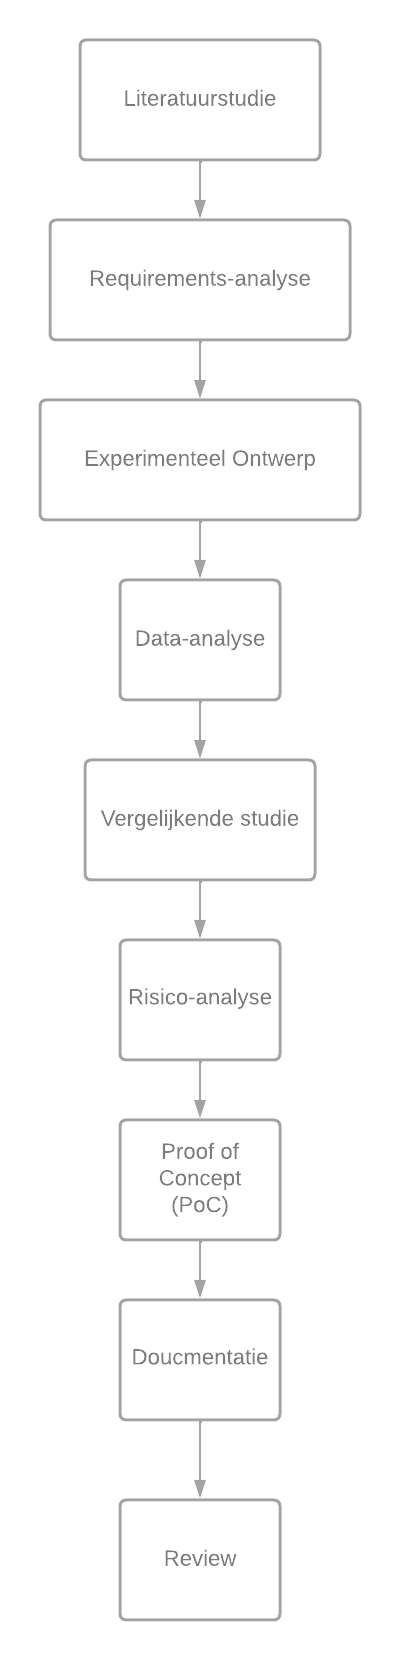
\includegraphics[width=0.3\textwidth]{Flowchart.png}
    \caption{Flowchart van het onderzoeksproces.}
    \label{fig:flowchart}
\end{figure}


%---------- Verwachte resultaten ----------------------------------------------
\section{Verwacht Resultaat en Conclusie}%
\label{sec:verwachte_resultaten}

De verworven kennis geeft momenteel aan dat de ontwikkeling van een hybride systeem, dat
MongoDB als NoSQL-database combineert met MySQL of PostgreSQL, de meest veelbelovende
benadering lijkt in termen van efficiëntie en kostenbeheersing voor kleine en middelgrote mode-e-
commerce platforms. Er wordt verwacht dat vervolgonderzoek diepere inzichten zal verschaffen die
van cruciaal belang zijn bij de keuze van het meest adequate databasemanagementsysteem. Dit
vervolgonderzoek zal de technische specificaties en operationele kostenfactoren grondig moeten
afwegen om een weloverwogen besluit te kunnen nemen.


%---------- References ----------------------------------------------



%%---------- Andere bijlagen --------------------------------------------------
% TODO: Voeg hier eventuele andere bijlagen toe. Bv. als je deze BP voor de
% tweede keer indient, een overzicht van de verbeteringen t.o.v. het origineel.
%\input{...}

%%---------- Backmatter, referentielijst ---------------------------------------

\backmatter{}

\setlength\bibitemsep{2pt} %% Add Some space between the bibliograpy entries
\printbibliography[heading=bibintoc]

\end{document}
